% Created 2025-07-12 Sat 14:07
% Intended LaTeX compiler: pdflatex
\documentclass[11pt]{article}
\usepackage[utf8]{inputenc}
\usepackage[T1]{fontenc}
\usepackage{graphicx}
\usepackage{longtable}
\usepackage{wrapfig}
\usepackage{rotating}
\usepackage[normalem]{ulem}
\usepackage{amsmath}
\usepackage{amssymb}
\usepackage{capt-of}
\usepackage{hyperref}
\author{Leonardo Bizzoni (899629)}
\date{\today}
\title{Relazione Laboratori Coderbot}
\hypersetup{
 pdfauthor={Leonardo Bizzoni (899629)},
 pdftitle={Relazione Laboratori Coderbot},
 pdfkeywords={},
 pdfsubject={},
 pdfcreator={Emacs 30.1 (Org mode 9.7.11)}, 
 pdflang={English}}
\begin{document}

\maketitle
\tableofcontents

\section{Trasformazione delle letture encoder in lunghezze degli archi percorsi}
\label{sec:orgb5719a4}
L'ottenimento dei tick misurati da entrambi gli encoder, sinitro e destro, viene fatto tramite le 2 istanze di `cbEncoder\textsubscript{t}` e leggendo il valore del parametro `ticks` periodicamente:
\begin{verbatim}
cbEncoder_t cb_encoder_left = { PIN_ENCODER_LEFT_A, PIN_ENCODER_LEFT_B, -1 };
cbEncoder_t cb_encoder_right = { PIN_ENCODER_RIGHT_A, PIN_ENCODER_RIGHT_B, -1};
\end{verbatim}

I parametri di queste 2 strutture vengono aggiornati tramite due funzioni callback `cb\textsubscript{encoder}\textsubscript{callback}\textsubscript{isrA}` e `cb\textsubscript{encoder}\textsubscript{callback}\textsubscript{isrB}` che vengono invocate quando il rispettivo canale, `A` o `B`, dell'encoder invia un interrupt per segnalare il cambiamento di livello (\emph{rising o falling edge}).

La conversione del valore in tick al suo corrispondente in millimetri percorsi viene fatto grazie a 2 costanti di conversione (\emph{una per encoder}) misurate in millimetri/tick.
Queste 2 costanti sono state trovate sperimentalmente cercando di far andare il coderbot in linea retta per un albitrario intervallo di tempo e misurando la distanza percorsa con un metro e osservando quanti tick erano stati misurati dai 2 encoder. Dopo aver ripetuto l'esperimento questi sono i risultati ottenuti:
\begin{center}
\begin{tabular}{lrr}
distanza percorsa & tick encoder sinistro & tick encoder destro\\
\hline
91mm & 828 & 832\\
109mm & 965 & 970\\
98mm & 909 & 882\\
105mm & 891 & 941\\
98mm & 908 & 851\\
104mm & 925 & 938\\
\end{tabular}
\end{center}
\begin{itemize}
\item Media mm/tick encoder sinistro:            0.11147909938205335
\item Media mm/tick encoder destro:              0.1117455840579235
\item Varianza tick encoder sinistro:            1.4429498891258886e-5
\item Varianza tick encoder destro:              3.7696146281431147e-6
\item Deviazione standard tick encoder sinistro: 0.003798618023868534
\item Deviazione standard tick encoder destro:   0.0019415495430565542
\end{itemize}

Come costanti di conversione abbiamo utilizzato le 2 medie (\emph{MillimeterFromTicks\textsubscript{Left}, MillimeterFromTicks\textsubscript{Right}}).
\subsection{Ciclo di controllo delle ruote}
\label{sec:org98722f5}
Il controllo delle ruote inizia leggendo il valore di velocità delle singole ruote impostato dalla task di controllo cartesiano. Questa lettura viene effettuata in sezione critica per evitare corse critiche dove la task di controllo cartesiano sovrascrive il valore di velocità mentre la task di controllo ruote cerca di leggerlo:
\begin{verbatim}
os_mutex_lock(state.speed.mutex);
// (mm/s) / (mm/tick) = (mm/s) * (tick/mm) = tick/s
f32 target_ticksXsec_left = state.speed.left / MillimeterFromTicks_Left;
f32 target_ticksXsec_right = state.speed.right / MillimeterFromTicks_Right;
os_mutex_unlock(state.speed.mutex);

// (tick/s) * (ms / 1000ms) = tick
u64 target_ticks_left = target_ticksXsec_left * ((f32)period_ms / 1000.);
u64 target_ticks_right = target_ticksXsec_right * ((f32)period_ms / 1000.);
\end{verbatim}
Il valore di velocità delle 2 ruote è dato in millimetri al secondo, mentre le 2 costanti, come detto in precedenza, sono misurate in millimetri su tick. Per trovare quindi il numero di tick che ci aspettiamo i 2 encoder abbiano misurato nell'intervallo tra l'attivazione precedente e la corrente è necessario dividere la velocità per la costante di conversione e scalare il risultato in base al periodo della task.

Usando un approccio a 2 task, una per ogni ruota, si potrebbe sostituire il mutex lock con un rwlock per evitare di bloccare inutilmente le 2 task di sola lettura di controllo ruote, anche se per una così breve sezione critica non porterebbe a grandi miglioramenti:
\begin{verbatim}
// nella task di controllo ruote
os_rwlock_read_lock(state.speed.rwlock);
  // .....
os_rwlock_read_unlock(state.speed.rwlock);

// nella task del controllore cartesiano
os_rwlock_write_lock(state.speed.rwlock)
  // .....
os_rwlock_write_unlock(state.speed.rwlock)
\end{verbatim}

La frequenza di attivazione di questa task è stata arbitrariamente impostata a \(50\text{Hz}\), con deadline uguale al periodo. Il runtime è stato impostato misurando sperimentalmente la durata della singola attivazione, la quale impiega in media \(19799\text{ns}\) con un picco massima misurato a \(178125\text{ns}\) da cui la decisione di arrotondare molto generosamente il WCET a \(2\text{ms}\).

Dopodiche viene determinato il nuovo duty cycle dei motori in base all'errore tra tick misurati dagli encoder e tick attesi, scalato in base alle costanti proporzionali `Kp\textsubscript{Left}`, `Kp\textsubscript{Right}` e con l'aggiunta dell'errore accumulato durante l'intera esecuzione della task, scalato in base alle costanti integrali `Ki\textsubscript{Left}`, `Ki\textsubscript{Right}`.
La nuova direzione è data dal segno del duty cycle:
\begin{itemize}
\item duty cycle negativo implica che il coderbot deve muoversi indietro
\item duty cycle positivo implica che il coderbot deve muoversi in avanti
\item duty cycle nullo implica che il coderbot restare fermo e quindi la direzione è irrilevante
\end{itemize}
\begin{verbatim}
i64 delta_left = target_ticks_left - state.tick.measured_left;
i64 delta_right = target_ticks_right - state.tick.measured_right;

accumalated_error_left += delta_left;
accumalated_error_right += delta_right;

duty_cycle_left = Kp_Left * delta_left + Ki_Left * accumalated_error_left;
duty_cycle_right = Kp_Right * delta_right + Ki_Right * accumalated_error_right;

motor_direction_left = duty_cycle_left < 0 ? backward : forward;
motor_direction_right = duty_cycle_right < 0 ? backward : forward;

duty_cycle_left = Clamp(Abs(duty_cycle_left), 0.1, 0.6);
duty_cycle_right = Clamp(Abs(duty_cycle_right), 0.1, 0.6);

cb_encoder_left.ticks = 0;
cb_encoder_right.ticks = 0;
cbMotorMove(&cb_motor_left, motor_direction_left, duty_cycle_left);
cbMotorMove(&cb_motor_right, motor_direction_right, duty_cycle_right);
\end{verbatim}

Durante i test di movimento lineare del coderbot, abbiamo osservato che, con valori di duty cycle elevati, la differenza tra i tick riportati dai 2 encoder variava significativamente. I tick misurati dall'encoder sinistro erano decisamente maggiori di quelli misurati dall'encoder destro, il che portava il robot a tendere verso la destra.
Dopo ulteriori misure abbiamo stabilito che impostare valori di duty cycle minori di `0.2` è equivalente ad un duty cycle nullo, viceversa impostando valori maggiori di `0.6`, il rapporto tra tick misurati e duty cycle non era più lineare. Per ovviare a queste 2 situazioni abbiamo quindi deciso di limitare il valore di duty cycle dei 2 encoder ai valori \(\left[0.1,0.6\right]\).
\begin{center}
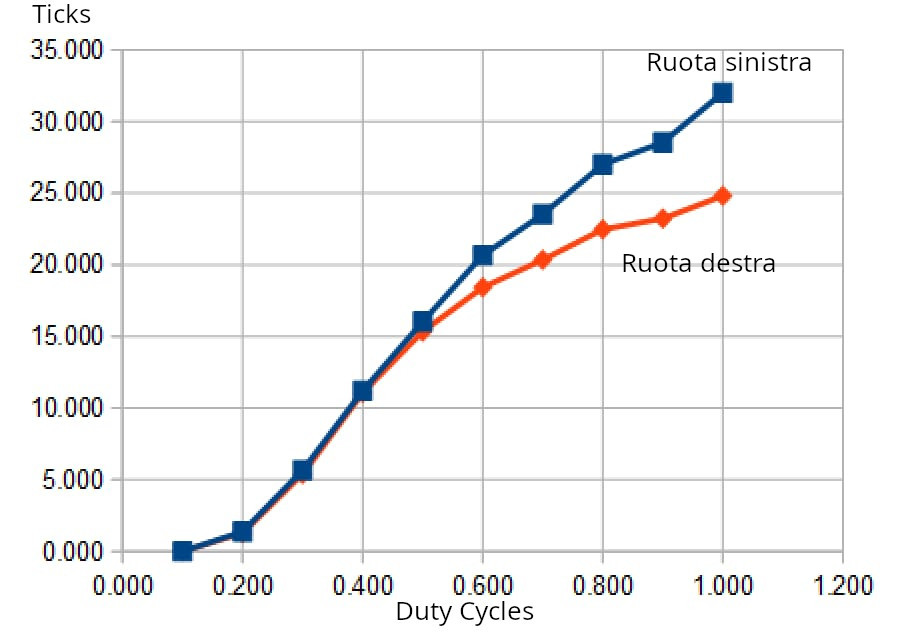
\includegraphics[height=200]{./img/pwm-ticks.jpg}
\end{center}

Trovare i valori delle costanti `Kp\textsubscript{Left}`, `Kp\textsubscript{Right}`, `Ki\textsubscript{Left}`, `Ki\textsubscript{Right}` è anch'esso stato fatto in maniera sperimentale separatamente.
Per le costanti proporzionali si è cercato di trovarle andado a modificarle con piccoli incrementi ad ogni esecuzione del programma cercando di aggiustarle per correggere l'andatura del robot. Abbiamo modificato il programma per prendere in input i valori delle costanti proporzionali da riga di comando ed eseguivamo ogni test facendo muovere il coderbot per 20 secondi, al termine dell'esecuzione controllavamo i tick complessivi misurati dai 2 encoder e la direzione verso cui il coderbot tendeva, in base a queste 2 osservazione andavamo ad aumentare:
\begin{itemize}
\item la costante destra se il robot tendeva a destra (\emph{oppure a diminuire la costante sinistra})
\item la costante sinistra se il robot tendeva a sinistra (\emph{oppure a diminuire la costante destra}).
\end{itemize}
Una volta trovate queste, si è passati alle costanti integrali che, analogamente, sono state regolate gradualmente con l'obiettivo di ridurre la discrepanza tra i tick desiderati e tick misurati.
Con le costanti proporzionali e le costanti integrali individuate, l'errore tra tick misurati e tick attesi si è ridotto all'intervallo \([-2,2]\) tick nella maggior parte delle attivazioni.

Per vedere l'output della task di controllo ruote è necessario ricompilare il programma passando il parametro `encoder` al build script:
\begin{verbatim}
./build.sh encoder
\end{verbatim}
\section{Odometria}
\label{sec:orgb8c87bf}
\subsection{Rappresentazione delle pose del robot}
\label{sec:orge782439}
\begin{center}
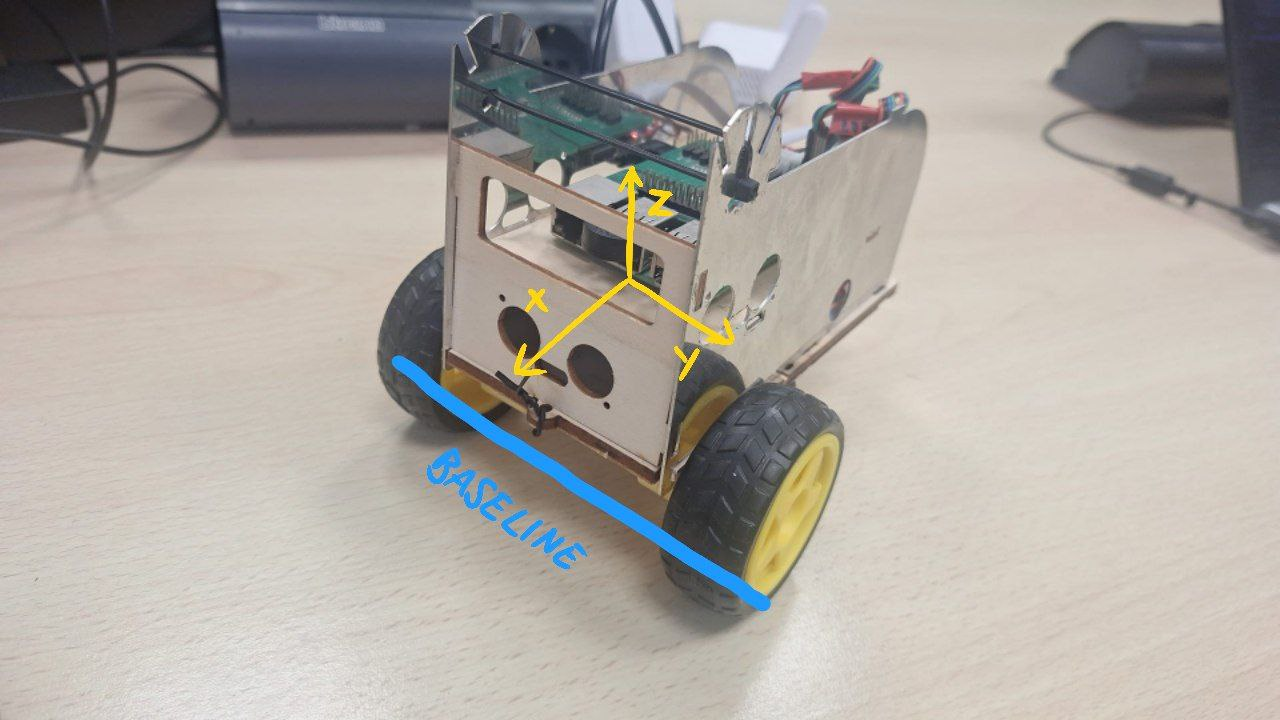
\includegraphics[width=300]{./img/coderbot-graph.jpg}
\end{center}

La pose del coderbot (\emph{la sua rotazione e posizione corrente}) viene modellata tramite una matrice \(3\times3\)  \(\text{pose}=\begin{bmatrix}R_{xx}&R_{yx}&P_x\\R_{xy}&R_{yy}&P_y\\0&0&1\end{bmatrix}\), dove:
\begin{itemize}
\item \(\bold R_{x}\) è il versore dell'asse X del sistema di riferimento attaccato al corpo del coderbot.
\item \(\bold R_{y}\) è il versore dell'asse Y del sistema di riferimento attaccato al corpo del coderbot.
\item \(\bold P\) è il vettore che indica la posizione del coderbot rispetto all'origine del sistema di riferimento attaccato al corpo del coderbot.
\end{itemize}
\subsection{Comportamento della task periodica}
\label{sec:org7e2259d}
Nella task di odometria vengono letti i tick misurati dagli encoder e, grazie alle costanti di conversione da tick a millimetri, si ottiene la distanza percorsa dal coderbot nel tempo percorso tra l'attivazione precedente e quella corrente della task di odometria:
\begin{verbatim}
f32 distance_left = ticks_left * MillimeterFromTicks_Left;
f32 distance_right = ticks_right * MillimeterFromTicks_Right;
\end{verbatim}

Similarmente alla task di controllo ruote, la frequenza di attivazione di questa task è stata arbitrariamente impostata a \(\sim33\text{Hz}\) (\(30\text{ms}\)), questo per dare una priorità maggiore alla task di controllo ruote avente periodo minore, e con deadline uguale al periodo. Il runtime è stato impostato misurando sperimentalmente la durata della singola attivazione, la quale impiega in media \(8431\text{ns}\) con un picco massima misurato a \(197917\text{ns}\) da cui la decisione di arrotondare molto generosamente il WCET a \(2\text{ms}\) come per il controllo ruote.

Sapendo la distanza percorsa dalle 2 ruote e la distanza tra di esse è possibile determinare l'angolo di rotazione rispetto al centro di istantanea rotazione:
\begin{verbatim}
f32 delta_theta = -(distance_left - distance_right) / BASELINE_MM;
\end{verbatim}
Per rispettare la convenzione secondo cui le rotazioni in senso antiorario hanno segno positivo, viene invertito il segno dell'angolo.
\subsubsection{Traiettoria rettilinea}
\label{sec:orgc92f689}
Se l'angolo \(\theta\) è minore di una certa soglia, da noi fissata a \(0.005\text{rad}\), allora dato che la rotazione misurata è prossochè nulla, possiamo approssimare il movimento ad una linea retta lungo l'asse delle \(X\) con modulo uguale alla media delle distanze percorse dalle 2 ruote.
L'operazione da applicare alla pose attuale del coderbot sarà una semplice traslazione lungo l'asse delle X, \(\text{pose}=\text{pose}\cdot\begin{bmatrix}R&P\\0^T&1\end{bmatrix}\) dove:
\begin{itemize}
\item \(R=I_2=\begin{bmatrix}1&0\\0&1\end{bmatrix}\)
\item \(P= \begin{bmatrix}(\text{distance left} - \text{distance right})/2\\0\end{bmatrix}\)
\end{itemize}
\subsubsection{Traiettoria curviliena}
\label{sec:orge1eb7ac}
Se l'angolo \(\theta\) è maggiore della soglia, questo indica che il coderbot sta effettivamente compiendo un movimento curvilineo, ruotando attorno a un centro di istantanea rotazione (\emph{CIR}). Questo CIR si trova lungo \(Y\) del sistema di riferimento del coderbot, ma traslato di una certa distanza `d`.
Il valore di `d` è dato dalla lunghezza dell'arco percorso da una delle 2 ruote, noi abbiamo deciso di considerare la ruota destra, diviso per l'angolo di rotazione. Dato che la lunghezza dell'arco è relativa alla ruota destra, è necessario sottrarre metà baseline per effettuare la traslazione rispetto al centro del coderbot:
\begin{verbatim}
f32 d = (distance_right / delta_theta) - (BASELINE_MM / 2);
\end{verbatim}

Per aggiornare la pose del coderbot, è stata applicata una rototraslazione `rt` ottenuta attraverso i seguenti passaggi:
\begin{itemize}
\item rotazione della matrice \(\text{t1}= \begin{bmatrix}1&0&0\\0&1&-d\\0&0&1\end{bmatrix}\), ovvero la matrice che esprime la posizione del CIR rispetto alla pose attuale del coderbot, di un angolo \(\theta\) rispetto l'asse Z del sistema di riferimento \emph{world}: \(R_z(\theta)\cdot\text{t1}\). Moltiplicando la pose del coderbot per questa matrice intermedia \(\text{pose}\cdot (R_z(\theta)\cdot\text{t1})\) stiamo allineando il coderbot con il CIR e vi stiamo applicando una rotazione rispetto l'asse Z.
\item applicazione di una traslazione inversa per riportare il coderbot alla posizione originale tramite moltiplicazione della matrice intermedia per \(\text{t2}= \begin{bmatrix}1&0&0\\0&1&d\\0&0&1\end{bmatrix}\), anch'essa definita nel sistema \emph{world}: \(\text{rt}=\text{t2}\cdot R_z(\theta)\cdot\text{t1}\).
\end{itemize}
Infine, la nuova pose del robot nel sistema \emph{body} è ottenuta applicando la rototraslazione `rt` alla pose corrente: \(\text{new pose} = \text{pose}\cdot\text{rt}\).
\subsection{Possibile idea di ottimizzazione}
\label{sec:orgeee593f}
Mantenere la pose del robot come una matrice \(3\times 3\) è superfluo dato che gli unici parametri di interesse sono:
\begin{itemize}
\item la posizione del robot nello spazio
\item l'angolo a cui si trova rispetto al mondo.
\end{itemize}
\subsubsection{Traiettoria rettilinea}
\label{sec:org913d27f}
Questo caso si semplifica al semplice incremento della componente X della posizione di \(\frac{(\text{distance left} - \text{distance right})}{2}\).
\subsubsection{Traiettoria curviliena}
\label{sec:org4c7050c}
All'inizio del programma, o anche dopo una sequenza di porzioni di rettilineo, il robot si trova ad un angolo nullo rispetto al mondo ed è quindi possibile rappresentare la rotoslazione come:
\begin{itemize}
\item traslazione della posizione lungo l'asse Y di \(d\) per trovare le coordinate del CIR \(\begin{bmatrix}X_\text{cir}=P.X\\Y_\text{cir}=P.Y-d\end{bmatrix}\)
\item traslazione dal CIR lungo l'asse Y di \(d\) con una rotazione \(\theta\) rispetto l'asse Z per trovare la posizione finale del robot \(\begin{bmatrix}X'=X_\text{cir}+d\sin(\theta)\\Y'=Y_\text{cir}+d\cos(\theta)\end{bmatrix}\)
\end{itemize}
\begin{center}
\includegraphics[height=100]{./img/odometry_opt_initial.jpg}
\end{center}

Nel caso generico in cui si sono susseguite porzioni di rettilineo e non, è necessario tenere traccia dell'angolo di inclinazione corrente del robot rispetto al mondo, qui chiamata \(\alpha\) (\emph{inizialmente inizializzata a \(0\)}):
\begin{itemize}
\item traslazione della posizione lungo l'asse Y di \(d\) con una rotazione di \(\alpha\) rispetto l'asse Z per trovare le coordinate del CIR \(\begin{bmatrix}X_\text{cir}=P.X-d\sin(\alpha)\\Y_\text{cir}=P.Y-d\cos(\alpha)\end{bmatrix}\)
\item traslazione dal CIR lungo l'asse Y di \(d\) con una rotazione \(\theta+\alpha\) rispetto l'asse Z per trovare la posizione finale del robot \(\begin{bmatrix}X'=X_\text{cir}+d\sin(\theta+\alpha)\\Y'=Y_\text{cir}+d\cos(\theta+\alpha)\end{bmatrix}\)
\end{itemize}
\begin{center}
\includegraphics[height=100]{./img/odometry_opt_generic.jpg}
\end{center}
\section{Generazione della traiettoria}
\label{sec:orgb8a0eec}
Il movimento del coderbot è stabilito da un percorso predefinito, il quale viene generato offline come una sequenza di punti in un piano. A runtime la task di controllo cartesiano cerca il punto della traiettoria più vicino alla posizione attuale, la quale viene aggiornata dalla task di odometria, confrontando solo i punti nell'intorno della posizione corrente (\emph{con una finestra di dimensioni \(10\) da entrambi le parti}), al fine di determinare un obiettivo intermedio da raggiungere.

La definizione della traiettoria avviene tramite concatenzazione delle primitive di generazione di archi di rotazione e rette.

Similarmente alla task di odometria, la frequenza di attivazione di questa task è stata arbitrariamente impostata a \(\sim 33\text{Hz}\) (\(30\text{ms}\)), per il medesimo motivo dell'odometria, e con deadline uguale al periodo. Il runtime è stato impostato misurando sperimentalmente la durata della singola attivazione, la quale impiega in media \(10836\text{ns}\) con un picco massima misurato a \(154948\text{ns}\) da cui la decisione di arrotondare molto generosamente il WCET a \(2\text{ms}\) come per le 2 precedenti task.

Dal momento che il controllore cartesiano ha il compito di guidare il coderbot nel seguire la giusta traiettoria, si ha la necessità di poter impostare la velocità delle singole ruote. Per evitare corse critiche con la task di controllo ruote, l'aggiornamento viene eseguito in sezione critica.
\subsection{Definizione della traiettoria}
\label{sec:org9f8ee40}
La generazione della traiettoria avviene offline tramite il metaprogram `gen-arcs` il cui compito è generare un file sorgente C contenente l'array di punti `waypoints` nello spazio cartesiano che rappresentano la triattoria del coderbot ed una costante rappresentante la lunghezza di tale array `N\textsubscript{POINTS}`. Il quale file viene incluso nel programma vero e propio.
Le funzioni `generate\textsubscript{arc}\textsubscript{points}` e `generate\textsubscript{line}\textsubscript{points}` popolano l'array `waypoints` con 50 punti l'una, rispettivamente per generare un arco di rotazione o una retta. Per poter generare traiettorie più complesse è stato necessario introdurre una nuova costante, chiamata `Chunks`, per indicare la posizione nell'array `waypoints` in cui inserire la nuova porzione di traiettoria. In alternativa sarebbe stato possibile trattare l'array `waypoints` come una lista dinamica di array:
\begin{verbatim}
typedef struct TrajectoryChunk {
  Points points[N_POINTS];
  struct TrajectoryChunk *next;
  struct TrajectoryChunk *prev;
} TrajectoryChunk;

// global = static
global struct {
  TrajectoryChunk *first;
  TrajectoryChunk *last;
} trajectory = {0};

// fn = static
fn void start(CmdLine *cmd) {
  Arena *arena = ArenaBuild(); // inizializza un arena allocator con:
                               // - default page commit size di 4KiB
                               // - default page reserve size di 4MB

  // alloca all'interno dell'arena abbastanza spazio per un TrajectoryChunk
  //   (la regione di memoria restituita è già zero-initialized)
  TrajectoryChunk *first = New(arena, TrajectoryChunk);
  // popola il chunk con i punti necessari per generare
  //   la traiettoria indicata
  generate_arc_points(first, 0, 900, 900, -90.f, 0.f);
  // aggiungi il chunk alla fine della linked list
  //   (non è necessario inizializzare ne trajectory.first
  //    ne trajectory.last, se ne occupa già la macro)
  DLLPushBack(trajectory.first, trajectory.last, first);

  TrajectoryChunk *second = New(arena, TrajectoryChunk);
  generate_arc_points(second, 1800, 900, 900, 180.f, 90.f);
  DLLPushBack(trajectory.first, trajectory.last, second);

  TrajectoryChunk *thrid = New(arena, TrajectoryChunk);
  generate_line_points(thrid, 1800, 1800, 900, 0.f);
  DLLPushBack(trajectory.first, trajectory.last, thrid);

  // .....
}
\end{verbatim}
\emph{Per maggiori informazioni riguardo all'arena allocator: \url{https://www.rfleury.com/p/untangling-lifetimes-the-arena-allocator}}.

L'approccio dinamico ci è sembrato inutilmente complesso per quello che ci serviva, quindi abbiamo deciso di optare per un semplice array `waypoints` di dimensione fissa `N\textsubscript{POINTS} * Chunks`, il che semplifica il codice di generazione di traiettorie complesse alle sole righe:
\begin{verbatim}
generate_arc_points(0, 900, 900, -90.f, 0.f);
generate_arc_points(1800, 900, 900, 180.f, 90.f);
generate_line_points(1800, 1800, 900, 0.f);
\end{verbatim}

La prima chiamata genera un arco rispetto ad un centro di rotazione posizionato in \((0cm,90cm)\) rispetto alla posizione iniziale del coderbot e di raggio \(90cm\). I restanti 2 argomenti indicano l'angolo iniziale del robot rispetto alla circonferenza e l'angolo finale/obiettivo.

\begin{center}
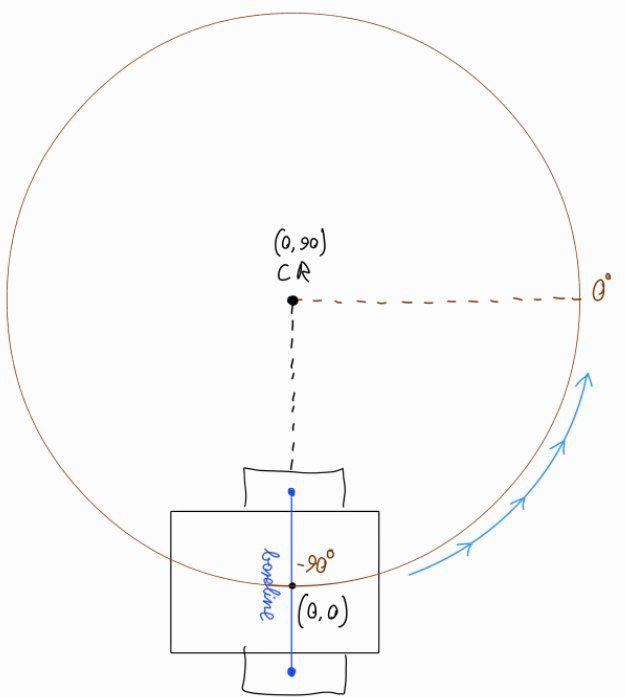
\includegraphics[height=200]{./img/gen_arc_example.jpg}
\end{center}

Similarmente la seconda chiamata genera un arco rispetto ad un centro di rotazione posizionato in \((180cm,90cm)\) rispetto alla posizione iniziale del coderbot e di raggio \(90cm\). La posizione di questo secondo centro di rotazione deve essere tale da poter continuare la traiettoria precedente ininterrottamente.
Infine l'ultima chiamata genera un porzione di traiettoria rettilinea con inizio alle coordinate \((180cm, 180cm)\) di lunghezza \(90cm\) e con un'inclinazione di \(0^\circ\).

La traiettoria finale sarà:
\begin{center}
\includegraphics[height=200]{./img/complex_trajectory_example.jpg}
\end{center}

Nonostante l'odometria indichi che il coderbot stia effettivamente seguendo la traiettoria prevista, questo non avviene realmente.
Il che è probabilmente dovuto ad un significativo slittamento delle ruote che porta il robot a rallentare o a bloccarsi ripetutamente nonostante le ruote continuino a girare. Di conseguenza, il sistema non è in grado di rilevare questa anomolia e prendere provvedimenti a riguardo.

Utilizzando una traiettoria semplificata, come un semplice arco di rotazione, abbiamo riscontrato maggiore successo, come si può ben vedere dal \href{./img/arc\_trajectory.mp4}{video allegato} (\emph{img/arc\textsubscript{trajectory.mp4}}) il robot segue correttamente la traiettoria descritta dalla chiamata:
\begin{verbatim}
generate_arc_points(0, -900, 900, 90.f, 0.f);
\end{verbatim}
\begin{center}
\includegraphics[height=200]{./img/arc_trajectory_example.jpeg}
\end{center}
\section{Gruppo di lavoro}
\label{sec:orga32bfa3}
La misurazione delle varie costanti sperimentali sono state fatte in collaborazione con: Camilla Cantaluppi, Fabio Lo Presti e Paolo Strianese.
Le restanti parti di sviluppo delle task di odometria e controllore cartesiano fino al completamento del progetto sono state svolte insieme a Camilla Cantaluppi (894557).
\end{document}
